\documentclass[a4paper, 12pt, article]{memoir}

\setlength{\footmarkwidth}{0em}
\setlength{\footmarksep}{0em}
\setlength{\thanksmarkwidth}{0em}
\setlength{\thanksmarksep}{0em}

\usepackage{fontspec}
\usepackage{amsmath}
\usepackage[tracking=true, nopatch=footnote]{microtype}
\usepackage{scalefnt}
\usepackage{csquotes}
\usepackage[main=english]{babel}

\usepackage{graphicx}
\usepackage{subcaption}
\usepackage{tikz} %for all basic options
\usepackage{tikz-qtree} %for simple tree syntax
\usepgflibrary{arrows} %for arrow endings
\usetikzlibrary{positioning,shapes.multipart} %for structured nodes
\usetikzlibrary{tikzmark}
\usepackage{tikz-qtree}
\usepackage{tree-dvips}

\setmainfont{Gentium Plus}
\setmonofont[Scale=0.8]{Noto Sans}

\babelprovide[import, onchar=ids fonts letters]{ancientgreek}
% \babelfont[ancientgreek]{rm}{Brill}
\babeltags{grc = ancientgreek}

\usepackage{hyperref}
\usepackage{linguex}
\setlength{\Exlabelsep}{0.5em}
\setlength{\SubExleftmargin}{1.5em}
\usepackage{paralist}
\usepackage{hyphenat}
\hyphenation{
  Κυ-ρι-α-κί-δη
  Θεσ-σα-λο-νί-κη
}

\usepackage[normalem]{ulem}
\RequirePackage{xcolor}
\definecolor{green}{RGB}{16,87,87} % rgb(16,87,87)
\definecolor{red}{RGB}{193, 11, 105} % rgb(193, 11, 105)
\definecolor{yellow}{RGB}{218,222,104} % rgb(218,222,104)
\definecolor{pink}{RGB}{243,179,145} % rgb(243,179,145)
\definecolor{blue}{RGB}{161,184,206} % rgb(161,184,206)

\RequirePackage{hyperref}%
\hypersetup{%
	colorlinks=true, % false: boxed links; true: colored links
	linkcolor=black,  % color of internal links
	citecolor=black,  % color of links to bibliography
	filecolor=black,  % color of file links
	urlcolor=black,
}

\usepackage[
  backend=biber,
  uniquename=init,
  giveninits,
  dashed=true,
  style=authoryear-comp
  ]{biblatex}
\addbibresource{./biblio.bib}


\title{Rethinking case attraction on Ancient Greek infinitive clauses}
\author{
  Caio B. A. Geraldes\thanks{Fundação de Amparo à Pesquisa do Estado de São
  Paulo.}
	\\\smallskip
	<\href{mailto:caio.geraldes@usp.br}{\texttt{caio.geraldes@usp.br}}>
}
\date{June 25, 2025}

\begin{document}

\maketitle

\chapter{Introduction}\label{chap:introduction} % (fold)

\paragraph{Good morning.} 
Nominal predicates and adjuncts modifying subjects of complement infinitive
clauses in Ancient Greek (AG) usually agree in case with their domain local
subject, which has morphological accusative case assigned in the
\emph{Accusativus cum Infinitivo} (\emph{AcI}) construction.
When the subject of the infinitive is not overtly expressed but the main clause
has a dative or genitive object which shares the reference of the infinitive
subject, these predicates or adjuncts may either occur in the accusative or ``be
attracted'' to the case of the main clause's object.

\ex.\label{gloss:base}
\a.\label{gloss:noattr}συμβουλεύει \textbf{τῷ Ξενοφῶντι ἐλθόντα} {εἰς Δελφοὺς}
ἀνακοινῶσαι {τῷ θεῷ} {περὶ τῆς πορείας}.\\
He advices Xenophon to go to Delphi and ask the god about the travel.
(Xen.\ \emph{Anab.} 3.1.5)
\b.\label{gloss:attr}ἀφῆκε \textbf{μοι ἐλθόντι} {πρὸς ὑμᾶς} λέγειν τἀληθῆ.\\
He allowed me to go and speak the truth in front of you.
(Xen.\ \emph{Hell.} 6.1.13)


The literature on the subject, on the more philological side, from
Port\hyp{}Royal (\cite{Lancelot1658,Lancelot1709}) up to the Cambridge
Grammar~(\cite{Boas2019}), have focused on listing the contexts in which
attraction may occur, whereas the transformational and minimalist approaches
of~\textcite{Lakoff1970}, \textcite{Andrews1971}, \textcite{Quicoli1982},
\textcite{Spyropoulos2005}, \textcite{Tantalou2003},
\textcite{Sevdali2006,Sevdali2013} have mainly occupied themselves with
proposing the structure that would allow the phenomenon to occur.
What factors influence the decision between either resolution
in~\ref{gloss:base} remains, however, largely unknown.

\paragraph{[Self-deprecatingly]} I myself have, in the last edition of this
same event, tried to present the distributional patterns that make the
attraction,~\ref{gloss:attr}, more likely, showing that there is strong
correlation between attraction and the classes of the matrix and infinitive
verbs and the relative distance and position of the controller and target of
agreement.

Furthermore, I argued that these factors were \emph{proxies} to unobserved
values, namely semantic and pragmatic features of the discourse setting, and
that even in the absence of seen contrasting factors, precisely the case in the
pair above~\ref{gloss:base}, the unseen discourse factors would be still causing
one resolution to be at the very least more likely.

\paragraph{[Introductingly]}
I wasn't, however, quite convinced about neither the methods, the data, and,
consequently, the quality of the results at which I had arrived.
The main reason for this distrust is the fact that there could be interaction
between the factors analysed which the methods employed were not well designed
to account for, at least not with the amount of data available.
To solve these shortcomings, we must take some steps back and build a model for
what is the linguistic nature of case attraction

The aim of this paper is to walk through the assumptions present in my own and
other's assessments of the phenomenon, as I believe most of them are in
themselves right, build from these assumptions a causal system and show how much
of this system is left unexplained with what we do know and, more importantly, I
believe, what we \textbf{can} know and measure about ancient languages in
general.


\chapter{The data}\label{chap:the_data} % (fold)

Before stepping into the framework and analysis proper, a brief word on the
empirical data supporting this research and any conclusion coming from it.
The dataset is composed of 343 sentences drawn from the Attic literary
\emph{corpus} and Herodotus.
The sentences were extracted from the Diorisis Corpus
(\cite{TheDiorisisAncientGreekCorpus,diorisis2021}) with help of the project's
querying tool, Diorisis Search (\cite{DiorisisSearch}).
Although comprehensive, the selection is by no means exhaustive.

Each sentence has been annotated for values of interest, including authorship,
literary genre, dialect as well as class of matrix and infinitive verb, class of
controller and target, distance between constituents, etc.
Parts of the annotation processes were conducted programmatically and later
checked manually.

Every model used in this work was processed using R (\cite{R}), the packages
\texttt{tidyverse} (\cite{tidyverse}), \texttt{dagitty} (\cite{dagitty}),
\texttt{ggdag} (\cite{ggdag}), and \texttt{rethinking} (\cite{McElreath2020}),
as well as the software Stan~(\cite{StanReferenceManual,StanUserGuide}).

% chapter The data (end)

\chapter{Nature of attraction}\label{chap:nature_of_attraction} % (fold)

In the most abstract way possible, case attraction in infinitive clauses,
exemplified by~\ref{gloss:attr}, is when two constituents, a controller and a
target, produced in different domains of a sentence, one of the domains
encompassing the other, covary in an specific feature, namely $[Case]$.
This satisfies the definition of agreement in Corbett's typological assessment
of the phenomenon across languages (\citeyear[pp.\ 4--7]{Corbett2006}).

The lack of covariation of the $[Case]$ feature, seen in~\ref{gloss:noattr}, is
generally understood as result of the application of \textbf{default} case
concord rules of Ancient Greek.
This assumes that the subject of infinitive clauses in Greek is always marked as
accusative, even when not overtly expressed, and that convert constituents are
also marked for $[Case]$ and its case is also available for nominal concord.

The facts that the target has a choice of controller (either the overt oblique or
de convert accusative) for agreement, that $[Case]$ is a non\hyp{}lexical
features, that the agreement is optional, and that the domain is non\hyp{}local
favours the interpretation that the agreement type of case attraction is less
canonical than the general agreement type of Ancient Greek, following the
criteria for canonical agreement in the same work of \textcite[pp.\
8ff.]{Corbett2006}.

If this assessment is sound, it is expected that attraction and
non\hyp{}attraction behave as competing agreement resolutions, the former being
less canonical and thus more likely to be conditioned.
Conditions concerning the semantic and pragmatic properties of the controller,
its precedence in relation to the target and the class of predication (i.e.:
class of the domain) have been identified by Corbett.
Although properties of the target were not shown to be favouring any resolution
in agreement mismatches in Corbett's survey, case attraction might be one
example of it, and I will hypothesize that properties of targets are competing
causes of non\hyp{}canonical resolutions.
A model of agreement in this framework may be represented as a direct acyclic
graph, in which \textbf{A}ttraction ($\simeq$ Agreement) is caused by features
of the \textbf{C}ontroller, \textbf{D}omain and \textbf{T}arget:

\begin{center}
	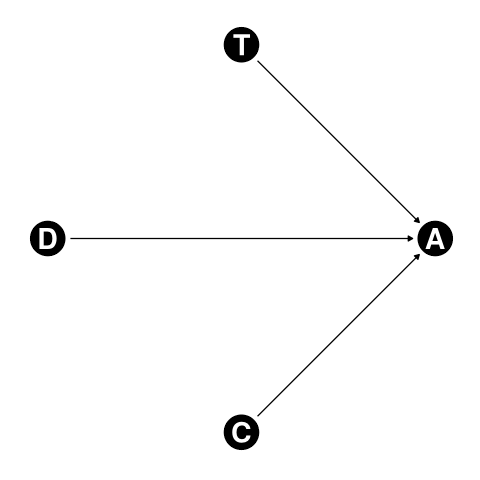
\includegraphics[width=0.60\textwidth]{figs/dag1.png}
\end{center}

These Controller, Domain and Target nodes represent clusters of linguistic
factors, some of which we may observe directly (part of speech of the target),
some might be implied (animacy) and some may remain unobserved (discourse
function, as Ancient Greek does not overtly marks focuses or topics in the
morphosyntax, at least not dependably).

The three factors previously shown to correlate to case attraction represent
each of these nodes:
\begin{compactitem}
	\item Copular infinitives imply a different domain of agreement, as they
		select different predication classes;
	\item Main verbs with semantic modality imply a different type of controller,
		as they have higher subjecthood;
	\item Word order and distance imply different status for the target, as
		targets more to the left of the sentence are both structurally closer to the
		controller and have a higher communicative function.
\end{compactitem}

% chapter Nature of attraction (end)

\chapter{The domain of attraction}\label{chap:the_domain_of_attraction} % (fold)

Firstly, \textcite{KG} and others have associated case attraction with sentences
in which the infinitival clause is a copular infinitive, einai or genesthai.
Should the class of the infinitive favour either resolution of agreement?
Probably not directly, as there is no reason linguistically it would.
Copular infinitives, however, have a double effect on the agreement ``causes'':
\begin{compactenum}
\item they filter the possible relations between controller and target, as those are
now more likely in primary predication, rather than secondary or appositive
relation;
\item this then delimits the option of target, making it more likely that they are nouns or adjectives, rather than participles.
\end{compactenum}

The these are known to affect agreement resolutions, and a couple of Hierarchies
have been proposed to predict when the less canonical resolution (also called
semantic agreement) is more likely to take place. The Agreement Hierarchy
(\cite{Corbett1979}) and Predicate Hierarchy (\cite{Comrie1975}) have also been
combined into the Agreement and Predicate Hierarchy shown
in~\ref{hierar:agreementpredicate2}:

\ex.\label{hierar:agreementpredicate2} Agreement and Predicate Hierarchies~(\cite[233]{Corbett2006}):\\
\begin{tikzpicture}[baseline=0pt]
    \node (attr) at (0, 0) {Attributive};
    \node (pred) at (2.5, 0) {Predicative};
    \node (predv) at (2.9, -0.4) {Verb};
    \node (predp) at (3.5, 1) {Participle};
    \node (preda) at (5, 2) {Adjective};
    \node (predn) at (7, 2.5) {Noun};
    \node (relp) at (5.6, 0) {Relative Pronoun};
    \node (perp) at (9.1, 0) {Personal Pronoun};
    \node (less) at (0, -1) {-};
    \node (plus) at (9.1, -1) {+};
    \draw[->, thick] (attr) to (pred);
    \draw[->, thick] (pred) to (relp);
    \draw[->, thick] (relp) to (perp);
    \draw[->, thick] (pred) to (predp);
    \draw[->, thick] (predp) to (preda);
    \draw[->, thick] (preda) to (predn);
    \draw[->] (less) to (plus);
    \draw[->] (plus) to (less);
    \node at (4.5, -1.5) {Likelihood of agreement with semantic justification};
\end{tikzpicture}


Adding this to our causal model, we may say that \textbf{A}ttraction is caused
both by whether or not the relation between the controller and target is
copular, and by the Part of Speech of the target, which is itself ``caused'' by
the type of relation (copulas select more nominal predicates on average), and
other unobserved properties of the \textbf{D}omain may also cause Attraction.


By applying the do-calculus~(\cite{Pearl2009}), we learn that:
\begin{compactitem}
	\item we can not estimate neither the total or direct effect of the infinitive
		verb being copular, as we can not close the non\hyp{}causal path $C \leftarrow D
		\rightarrow A$;
	\item the direct and total effect of the part of speech class requires us to
		adjust the correlation by $C$, so that we block the non\hyp{}causal path $P
		\leftarrow C \leftarrow D \rightarrow A$.
\end{compactitem}

\vfill
\clearpage


\begin{figure}[!h]
\centering
\begin{minipage}{.45\textwidth}
  \centering
  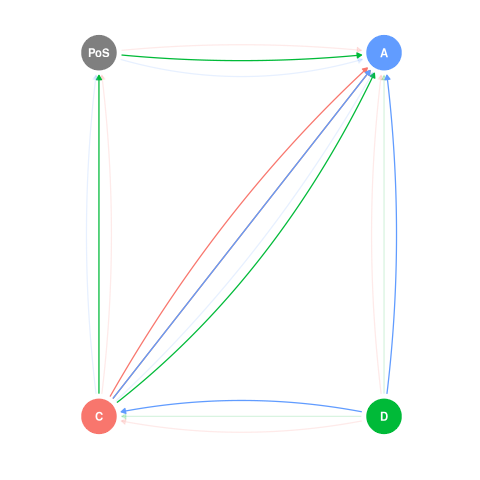
\includegraphics[width=\linewidth]{figs/dag2b.png}
  \captionof{figure}{Open causal paths between $C$ and $A$. The green node is
	unobserved. The blue path is non\hyp{}causal and can not be closed.}
  \label{fig:openpaths_c_a}
\end{minipage}%
\hfill
\begin{minipage}{.45\textwidth}
  \centering
  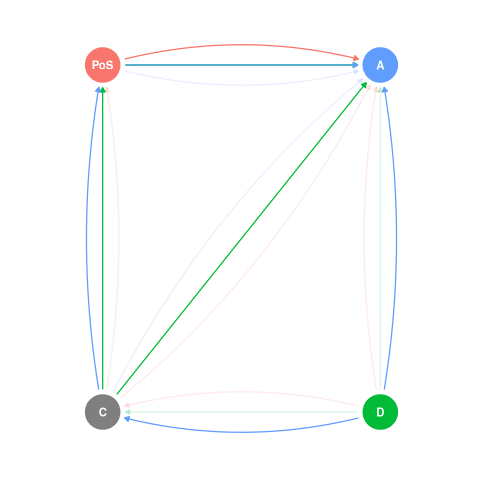
\includegraphics[width=\linewidth]{figs/dag2a.png}
  \captionof{figure}{Open causal paths between $PoS$ and $A$. The green node is
	unobserved. The blue path is non-causal and must be closed by adjusting for
	$C$, which also closes the green path.}
  \label{fig:openpaths_pos_a}
\end{minipage}
\end{figure}

To estimate the effect of $PoS$ over Attraction, we can use the generalized
linear model below.
We can control for Author, as there is no reason to believe that any author from
the corpus prefers copulas or any type of target.
As it is usually agreed that typological hierarchies increase their effect
monotonically by each of their nodes, but we do not know if their effect should
be linear or not, a Dirichlet prior is suitable to express the effect of Part of
Speech.
We coarse the base likelihood of case attraction to be negative as we assume
that it is the non\hyp{}canonical agreement resolution, meaning it should be
less likely to occur.

\begin{align*}
	\text{A} &\sim \text{Bernoulli}(p_i)\\
	\text{logit}(p_i) &= \alpha + \beta_{PoS}\sum^{PoS_i-1}_{j=0}{\delta_j} +
	\beta_{C}\text{C}_i  + \beta_{Auth_i}\\
	- \alpha &\sim \text{LogNormal}(0, 1)\\
	\beta_{PoS} &\sim \text{Normal}(0, 1)\\
	\delta &\sim \text{Dirichlet}(2)\\
	\beta_C &\sim \text{Normal}(0, 1)\\
	\beta_{Auth_j} &\sim \text{Normal}(\overline{\beta}_{Auth}, \sigma_{Author})\\
	\overline{\beta}_{Auth} &\sim \text{Normal}(0, 1)\\
	\sigma_{Auth} &\sim \text{Exponential}(1)
\end{align*}

\noindent The priors are fairly flat, as there is no reason to believe we have weak or
strong relationships in agreement phenomena.
$\beta_{PoS}$ is the general effect of the part of speech over the likelihood of
Attraction, it is slightly negative, and $\delta$ is a vector with values
denoting how much going up from Participle to Adjective to Noun increases
$\beta_{PoS}$.
Participles do not change the effect, Adjectives add $\delta_1$ and Nouns add
$\delta_1 + \delta_2$, meaning that the effect is expected to be cumulative.

The estimated effects are described in the following table and plot.

\begin{center}
	\begin{tabular}[c]{lllll}
	\toprule
	Effect				&	Mean	&	SD		&	5.5\%	&	94.5\%\\
	\midrule
	$\beta_{PoS}$		&	-0.13 &	0.33	&	-0.66	& 0.40\\
	$\delta_{Adj}$  &	0.49	& 0.22	&	0.14	& 0.85\\
	$\delta_{Noun}$	&	0.51	& 0.22	&	0.15	& 0.86\\
	\bottomrule
	\end{tabular}

	\bigskip
	\begin{tabular}[c]{llllll}
	\toprule
	PoS					&	Cumulative effect		&	Mean	&	SD		&	5.5\%	&	94.5\%\\
	\midrule
	Participle	& $\beta_{PoS}$		& -0.13 &0.33& -0.66&  0.40\\
	Adjective		& $\beta_{PoS} + \delta_{Adj}$  &0.36 & 0.44 & -0.33&  1.06\\
	Noun				& $\beta_{PoS} + \delta_{Adj} + \delta_{Noun}$  &0.87& 0.33&  0.32 & 1.38\\
	\bottomrule
	\end{tabular}
\end{center}


\begin{center}
	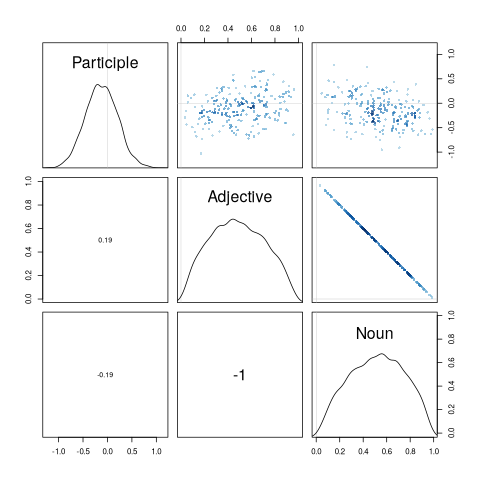
\includegraphics[width=0.75\linewidth]{figs/model3_banddelta.png}
\end{center}

To put it into words, the data favours the idea that the Agreement and
Predication Hierarchy holds for case attraction in Ancient Greek case
attraction: as the target becomes more ``nominal'', the likelihood of attraction
increases from slightly negative up to highly positive.
Notice that the model assumes that the effect of adjectives and nouns are
negatively correlated, meaning that it does not discounts the possibility that
the bulk of the effect is in the passage from Participles to Adjetives, and
going further up to a Noun makes little difference.


\chapter{The controller of attraction}\label{chap:the_controller_of_attraction} % (fold)

Another association is that between case attraction and impersonal verbs.
I have, however, shown that this association does not exist with every single
impersonal verb, and that the verb δοκέω almost never heads a sentence with case
attraction.
The impersonal verbs which are actually associated with case attraction are
those carrying modal semantics, such as ἐξαρκεῖ and ἔξεστί.
Is it likely that the nature of the matrix verb directly affects the choice of
agreement? I don't think so, but it may indirectly do, by defining which
features the controller of agreement, the oblique object, has.
These verbs have very little semantic information and the theta role and
grammatical function of their oblique object seems to depend on the infinitive
verb.
We may say that σοι in~\Next, for example, is the subject of the sentence
(a quirk subject of sorts) and has the thematic role of agent, much in contrast
if the sentence was constructed with a verb of order or advice like συμβουλέυω.


\ex. ἀλλ᾽ ἐξαρκῇ σοι τὰ ἔργα αὐτῶν ὁρῶντι σέβεσθαι καὶ τιμᾶν τοὺς θεούς.\\
But it is enough for you to look at these deeds and respect the gods. 
(Xen.\ \emph{Mem.} 4.3.13) 


% A ⊥ Genre | PosV


% chapter The controller of attraction (end)

\chapter{The target of attraction}\label{chap:the_target_of_attraction} % (fold)


Finally, it has been long been proposed that case agreement is more likely when
controller and target are very close to each other, and the likelihood
diminishes as it grows.
I have previously showed that, although very much associated, long distance
between controller and target is not a dependable predictor for lack of
attraction, but that precedence of the target in relation to the controller
seems to demand case attraction, such as in~\Next.

\ex.ὡς \textbf{ἀγαθοῖς} τε \textbf{ὑμῖν} προσήκει εἶναι.\\
That you may be good people. (Xen.\ \emph{Anab.} 3.2.11)

As with the previous factors, we must ask: are distance and precedence directly
causing case attraction, or are they indirect causes?
Longer distances have been show to favour non-canonical agreement resolutions in
other languages, such as with personal pronouns agreeing with committee nouns in
English, which are more likely to be plural the further away from their
controller.
This is the very opposite of what is being proposed for case attraction: the
canonical agreement (the local one) is the one becoming more likely as farther
away the target is from the controller.

% chapter The target of attraction (end)

\renewcommand*{\mkbibnamefamily}[1]{\textsc{#1}}
\printbibliography%
\renewcommand*{\mkbibnamefamily}[1]{#1}

\end{document}
